

Supportive hand contacts are essential for mastering every-day life tasks, for 
example, when reaching for a glass on the highest shelf humans typically have to 
use the other hand to support their body on the kitchen table. In such 
scenarios, the motion of the body and both arms have to be perfectly 
synchronized to successfully perform the reaching motion and to simultaneously 
ensure the postural stability. However, little is known about the underlying 
processes that govern the motion of the human body during and after the learning 
of these kinds of concurrent motor skills. To study the effect of supportive 
contacts on motor control of reaching, an innovative full-body experimental 
paradigm was established that extends current experimental methods to a more 
ecological setting. The task of the subjects was to reach with their right arm 
for a distant target on a screen while postural stability could only be 
maintained by establishing an additional supportive hand contact with their left 
arm. To examine adaptation, non-trivial postural perturbations of the subjects' 
support base were systematically introduced. A novel probabilistic trajectory 
model approach was employed to analyze the correlation between the motions of 
both arms. We found that subjects adapted to the perturbations by establishing 
supportive hand contacts that were dependent on the location of the reaching 
target. Moreover we found that the trunk motion adapted significantly faster 
than the motion of the arms. However, the most striking finding was that 
observations of the initial phase of the left arm or trunk motion (100-400 ms) 
were sufficient to faithfully predict the complete movement of the right arm. 
Overall, our results suggest that the goal-directed arm movements determine the 
supportive arm motions that ensure postural stability and that adaptation 
happens on different time scales, where the motion of heavy body parts adapts 
faster than light arms. 

\section{Introduction}
Most of our every day motor skills involve strict control of postural stability 
in parallel to the execution of the primary motor task. A great deal of these 
tasks also require additional supportive hand contacts beside the feet that are in contact with the ground. An example task is the reaching for a glass on 
the highest kitchen shelf when we typically have to use the other hand to 
support the body by leaning on the kitchen counter. To successfully perform such a reaching 
motion and to simultaneously ensure the postural stability, the motion of the 
body and both arms have to be perfectly synchronized and coordinated.

In general, supportive hand contacts increase the stability during balancing and 
complement humans' sophisticated motor abilities, e.g., in reaching for distant 
objects, during acrobatics or simply to navigate in the dark through leaning 
against a wall\cite{cordo1982properties, jeka1994fingertip, 
balasubramaniam2002dynamics, dickstein2003effects}. 
%Balancing is known as the most basic motor control problem \cite{reed1982outline, Hofsten1993prospective}. 
Like the ability to balance, the utilization of supportive hand contacts has to be learned \cite{reed1982outline, Hofsten1993prospective}. 
At about two months infants are able to balance and turn their head to focus on 
interesting events; at six months they can balance in sitting position; at eight 
months infants already learn how to balance on hands and knees during crawling; 
at ten months they start walking with support from hanging on a table or a 
couch; and at about one year infants already know how to balance on two feet and 
walk independently across the room \cite{adolph2002learning, adolph2006motor}. 
While it is known that people develop optimal motor control strategies both for 
postural stability and manipulation \cite{pai1997center, scott2004optimal, 
todorov2004optimality}, it is unclear how these two distinctive motor tasks 
relate to each other and how their relationship affect the learning of novel motor 
skills or when re-establishing motor abilities in novel environments. A thorough 
understanding of these issues is of particular interest for the field of 
rehabilitation, where correlations between the primary motor tasks and the 
underlying supportive motor actions could be exploited in progress monitoring 
and novel pre-tests of motor dysfunctions \cite{duncan1990functional}. 

%Despite the obvious importance, little is known about the underlying motor 
%control processes that govern the motion the human body during and after 
%learning of these kind of concurrent motor skills. 

Many of previous studies 
either focus on control of postural stability \cite{horak1986central, 
kuo1995optimal, winter1995human, Lockhart2007}, study adaptation of arm reaching 
in confined lab environments \cite{shadmehr1993postural, wolpert1995arm, d2006control, 
diedrichsen2010coordination, berger2013differences}, or study situations when 
postural stability and arm reaching are only indirectly related 
\cite{flash1990human, stapley1999does, slijper2000effects, babivc2014effects, 
johannsen2007effects}.
%
In our study we propose an innovative full-body experimental paradigm 
(\FigureAbbr 
\ref{fig:subFigContactLocationsAllSubjects}A) that extends current experimental 
methods to a more ecological setting where postural stability and manipulation 
skills are tightly interrelated and interdependent to each other. We hypothesize that the arm reaching motions determine the supportive hand 
contact strategies and that both motor tasks adapt during training. In 
particular, we assume that these two motor tasks are correlated which is 
reflected in synchronized motor executions and a significant correlation between 
target locations and supportive hand contacts. To effectively elaborate on these hypotheses we designed an experimental paradigm where we
asked $20$ 
healthy subjects to reach with their right arm for a target displayed on a 
screen while using their left arm to maintain postural stability by leaning on a 
table in front of them.
Non-trivial postural perturbations 
of the subjects' support base were systematically introduced to examine 
adaptation and a novel probabilistic trajectory model approach was employed to 
analyze the correlations between the supportive arm motion and the motion of the 
arm to reach for the distant target.


\begin{figure}[t]
\centering
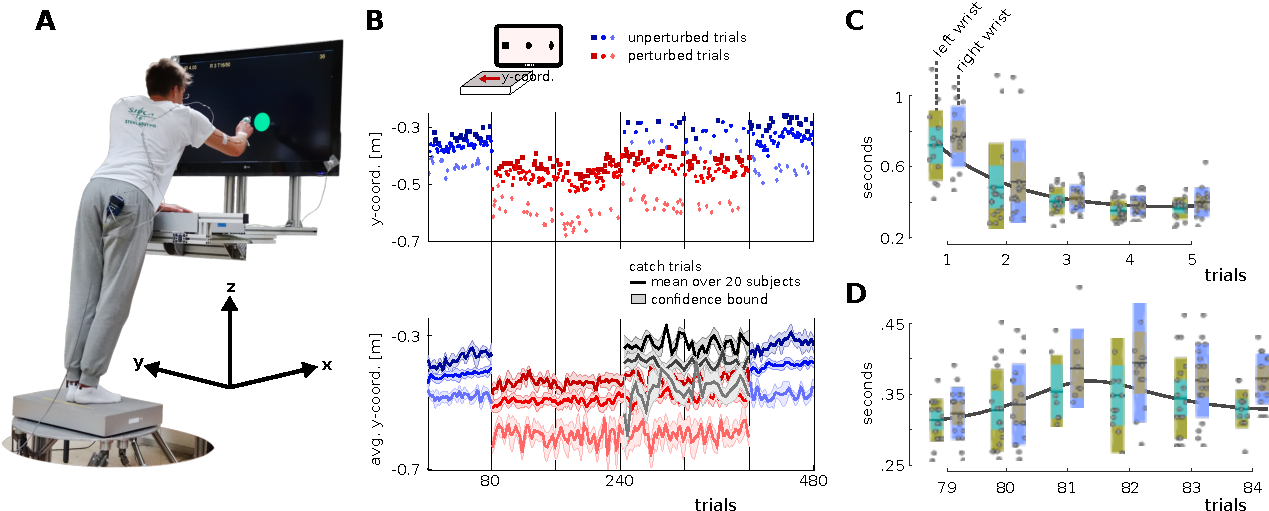
\includegraphics[width=\textwidth]{Elmar/picsClean/Fig1ExperimentContactsOnsets}
%\label{fig:subfig2}
 \caption{\textbf{Experiment, target dependent contacts and synchronized arm motions.} \textbf{A)} Experimental setting. 
 \textbf{B)}  The top row shows contact locations for a single representative subject 
 and the bottom row shows the mean and the confidence bound over all $20$ participants. 
 The first $80$ trials and the last $80$ trials are unperturbed sessions. 
 Catch trials were initiated during trials $240$ to $400$ and are denoted by the black lines in \textbf{B}.
%  
%  Note that during catch trials the contact 
%  location immediately switches back to the unperturbed behavior. This can be explained by the fact that the contact location 
%  is a result of both, the trunk motion (which shows strong negative after effects) and the left wrist motion (were we could not find these effects). 
%  Another finding is that contact locations are target correlated denoted by the three lines in \textbf{B} . 
 \textbf{C)} Illustration of the movement onsets of the wrists for the first five trials. 
 \textbf{D)} Movement onsets for the first six trials transitioning to the perturbed session. 
}
\label{fig:subFigContactLocationsAllSubjects}
\end{figure}


%NOTE Implications will be moved to the discussion 
\section{Results}%\label{sec:methods}

After a random interval of one to 
three seconds, the target was presented on the screen at one out of three possible locations (i.e., randomly at the left, the center or the right side on a horizontal bar). We motivated the subjects 
through a monetary reward that was proportional to the time needed to reach for 
the target. This reward was displayed after the target was reached. The number zero was displayed if the trial time exceeded two seconds. 
In our results, we focused on the y-coordinate of the contact locations 
as it corresponded to the direction of the translational 
perturbation. This is indicated by the arrow labeled by $y$ in \FigureAbbrP \ref{fig:subFigContactLocationsAllSubjects}. 

%\subsection*{Humans pick task dependent contact locations} 

\subsection{Subjects chose task dependent contact locations} 

Analysis of 
variance (ANOVA) showed a significant effect in the left hand contact location between 
sessions when the subjects were perturbed and unperturbed during reaching toward 
targets displayed on screen, $F(1,19) = 113.632$, $p < 0.001$, $\eta_p^2 = 0.857$.

The post-hoc analysis showed that the left hand contact location was significantly 
different between reaching toward all three distinctly positioned targets in 
perturbed, $t(19) = 6.85 \text{ to } 11.58$, $p < 0.001$, and in unperturbed trials, $t(19) = 
6.78-12.21$, $p < 0.001$.

There were also significant differences between means of contact locations for 
each target between perturbed and unperturbed trials (target one, $t(19) = 10.07$, $p 
< 0.001$, $d = 2.01$; target two, $t(19) = 10.22$, $p < 0.001$, $d = 2.38$; target three, $t(19) = 
11.51$, $p < 0.001$, $d = 3.25$), see Supplementary \FigureAbbr 
\ref{fig:SubFigANOVAContacts}.



%it is known that preparation actions depent on future actions cite Schack
%here we investigate is contacts change depdent on future goal-directed reaching

%We found distinct contact locations for each of the three tested targets during 
%the unperturbed cond. and the perturbed condition %Figxx (a-b)

%Subject frame reports numbers that are a result of both, trunk and left arm movements. 

Further, we analyzed individual sessions of unperturbed, perturbed and catch 
trials. We compared them with each other to determine whether there are any 
differences between contact locations and for which target positions they apply.

The first $80$ trials out of $480$ training trials were unperturbed. We found that 
there was a significant effect of target locations on the supportive contact 
locations in these first $80$ trials, $F(1.11,21.14) = 104.61$, $p < 0.001$, $\eta_p^2 = 
0.846$, see \FigureAbbr \ref{fig:subFigContactLocationsAllSubjects}B. Post-hoc tests using the Bonferroni correction \cite{bland2000introduction} revealed 
that there was significant difference in chosen supportive contact location 
between all three targets ($t(19) = 6.92 \text{ to } 11.66$, $p < 0.001$).

After the initial training phase, all subjects had to adapt to translational 
perturbations of the support base. Note that to compare the contact locations and the 
marker trajectories of perturbed and unperturbed trials, we corrected all sensor 
readings by the motion of the moving base. We refer to this correction as the 
\textit{subject frame}. Later we will introduce \textit{shoulder frames} to 
separate adaptation in the trunk and in the arms. Again, we found that there was a 
 significant effect of the target location on the contact location over all perturbed 
 trials, $F(1.33,25.27) = 116.39$, $p < 0.001$, $\eta_p^2 = 0.86$, see trials 
 $81 \text{ to } 240$ in \FigureAbbr \ref{fig:subFigContactLocationsAllSubjects}B. Post-hoc 
tests showed a significant difference in the chosen supportive contact location 
 among all three targets ($t(19) = 6.85 \text{ to } 11.58$, $p < 0.001$).

Consolidation of the postural control strategies was tested through randomly 
initiating unperturbed trials (catch trials). In the last phase of perturbed 
trials (trials $320$ to $400$), where adaptation can be assumed to be converged, 
the perturbation was deactivated for $30$ random catch trials. When comparing initial training 
trials with catch trials post-hoc tests showed no significant difference for all 
three targets, target one ($t(18) = -1.99$, $p = 0.062$, $d = -0.74$), target two 
($t(18) = -3.28$, $p = 0.004$, $d = -1$) and target three ($t(18) = -1.03$, $p = 
0.315$, $d = -0.39$).
%
Comparison of perturbed and catch trials showed significant differences in 
contact locations for all three target locations ($t(18) = -11.24 \text{ to } -12.97$, $p < 
0.001$, $d = -2.44 \text{ to } -1.93$).
%
For the washout, no significant difference was observed between contact 
locations for individual targets when comparing catch and final trials $401 \text{ to } 480$ 
($t(18) = -1.59 \text{ to } 1.28$, $p = 0.13 \text{ to } 0.22$, $d = -1 \text{ to } -0.39$).



%Conclusion 
In summary, we found that subjects chose distinct contact locations dependent on the 
target location on the screen. Catch trial tests revealed that the participants 
learned specialized control strategies for unperturbed and perturbed conditions. 
However, whether the distinct contacts result from trunk or left arm adaptations 
can not be answered from looking at contact locations only. That 
requires a more detailed analysis of the temporal profiles for which we will 
introduce a probabilistic trajectory model. 

%Implication


\subsection{Supportive and goal-directed movements synchronize}

Decreasing reaction times are an indicator for adaption of a pre-processing 
phase \cite{klatzky1995planning}. In line with this, we found that the movement onsets of the left 
and the right wrist synchronize within $3-5$ trials in the unperturbed training 
phase (left wrist: $323 \, \pm 44 \textrm{(SD)}$ ms, right wrist: $335 \, \pm 46$ ms) and when the 
perturbations are experienced for the first time (left wrist: $333 \, \pm 48$ ms, right wrist: $342 \, \pm 49$ ms). 
For the first six trials, the onsets of all subjects and the computed means and standard deviations (SD) are illustrated in \FigureAbbr \ref{fig:subFigContactLocationsAllSubjects}C-D. 

No significant dominance of the supportive left arm motion 
over the right arm reaching movements was found in the data. 
This is shown in an illustration of movement onsets of all subjects in Supplementary \FigureAbbr \ref{fig:subFigWristPriorities}. 
%Conclusion 
%Implication

%Details to the statisticss
%$323 \, \pm 44, right wrist: $335 \, \pm 46$ for trials $10-80$
%$333 \, \pm 48$ ms, right wrist: $342 \, \pm 49$ ms for trials $90-160$ 


\subsection{Modeling joint distributions over limb trajectories}
%limb trajectories are recorded time series. Linear and non-linear time series models have been used. Autoencoder 
%Human motor variability can be encoded in probabilistic models, cite wolpert, rueckert pmp
Reaction times are sensitive to signal noise, need to be verified through visual inspection and 
allow only for a limited view on the functional mechanisms during skill learning. 
As an alternative to reaction time studies, we propose to analyze adaptation on 
a trajectory basis. 
%
For that we developed a probabilistic trajectory model (PTM) that encodes a 
joint distribution over multiple limb trajectories and over multiple coordinates 
like x, y, z components of three-dimensional marker data. Here, we give a brief 
summary of PTMs and for a precise mathematical definition we refer the reader to 
the Methods section. 

\begin{figure}[t]
\centering
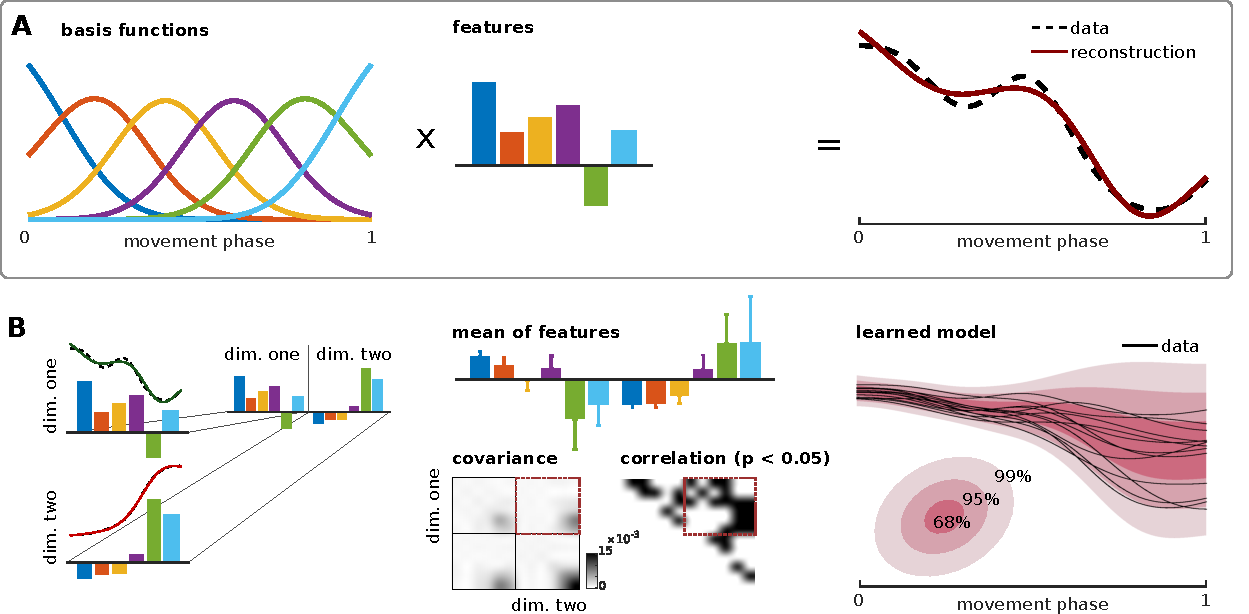
\includegraphics[width=1\textwidth]{Elmar/picsClean/AProbModelofMotionApproach1}
%\label{fig:subfig2}
 \caption{\textbf{Probabilistic model of trajectories, from a feature space (left column) to trajectories (right column):}  
 \textbf{A)} Generative model. 
 Equally spaced (radial) basis functions are amplitude scaled by a feature vector to approximate a one-dimensional trajectory. 
 A movement phase substitutes time to model trajectories of different lengths. 
 In the inverse direction, feature vectors are computed given the input trajectories using, e.g., standard linear regression techniques or 
 iterative variational approaches like expectation-maximization. 
 \textbf{B)} Learning the correlations between multi-dimensional input trajectories. 
 Feature vectors computed from multiple input trajectories are concatenated 
 and the mean and the covariance are computed from multiple trials (or subjects). 
 The learned correlation in the center panel is the key features for computing predictions from 
 partial observations. The distribution over trajectories is shown in the right panel. 
}
\label{fig:model}
\end{figure}

The main feature of the model is that it captures the correlations between 
individual input dimensions. The model builds on a linear function approximator 
using radial basis functions with fixed means and variances. 
The amplitudes are scaled by learnable features. Now both, the basis functions and the features,  
form a linear generative model of a trajectory, i.e., $\vec \tau = \vec \Phi \, 
\vec w$ (with the trajectory $\vec \tau = [y_1, y_2, ..., y_t]$, time-varying observations $y_t$, basis functions 
in $\vec \Phi$ and feature weights $\vec w$). \FigureAbbr 
\ref{fig:model}A shows the encoding of a single trajectory using classical radial 
basis functions. Note that the model is linear in the feature space, however it 
can capture non-linear dependencies in the trajectory space (through non-linear basis functions). The model's complexity is controlled 
through the number of basis functions. For the reaching experiments 
ten Gaussian distributions per dimension were found to be sufficient, see Supplementary \FigureAbbr \ref{fig:subFigNumGaussians}.

The feature vector 
$\vec w$ can be learned in the most simple case through standard linear 
regression or in more sophisticated models through one of the many existing 
variational inference methods \cite{Rueckert2015}. 

A PTM encodes multiple input dimensions through a concatenated feature vector (a 
two-dimensional example is illustrated in \FigureAbbrP 
\ref{fig:model}B). This concatenated feature vector scales the contribution of an 
\textit{extended} basis function matrix. Thus, the only difference to standard 
radial basis functions is a clever arrangement of basis functions and feature 
vectors to represent multiple input dimensions in one model. 
 
To model a distribution over trajectories the mean and the covariance over multiple trials are computed from the 
inferred feature vectors (e.g., through linear regression). An example is shown 
in the center panel in \FigureAbbr \ref{fig:model}B. The mean and 
the covariance encode a distribution over trajectories in the feature space and 
through the relationship $\vec \tau = \vec \Phi \, \vec w$, the distribution can 
be mapped (back) to the time domain. It is worth mentioning that a PTM can 
represent trajectories of varying lengths by substituting time by a movement 
phase. The last panel in \FigureAbbr \ref{fig:model}B shows an 
illustrative example of a trajectory distribution and the corresponding input 
trajectories using a movement phase.    

%Conclusion  
To conclude, the advantage of the presented time-series model is that it can be formulated as a 
generative probabilistic model for which many learning algorithms and similarity 
measures exist. The model can encode the signal variation and can be used to 
compute operations like predictions, model comparisons or trial likelihoods. 
These operations are explored in the present study on postural control with supportive 
contacts. 
%Implication the model can be used on an time series data and captures the correlation. Examples are EMG recordings, EEG channel encoding, temperature or force profiles, etc.   


\subsection{Supportive contacts predict goal-directed movements}

The learned and represented correlation of multiple limb trajectories can be 
exploited in computing predictions. This feature is used here to investigate if 
left wrist trajectories can predict the right wrist 
reaching trajectories. To separate the contributions of the trunk and the left 
arm, we transformed the wrist marker trajectories to a \textit{shoulder frame}. 
For that the wrist positions in the subject's coordinate frame were additionally 
corrected by the time-varying shoulder marker positions. 

\begin{figure}[t]
\centering
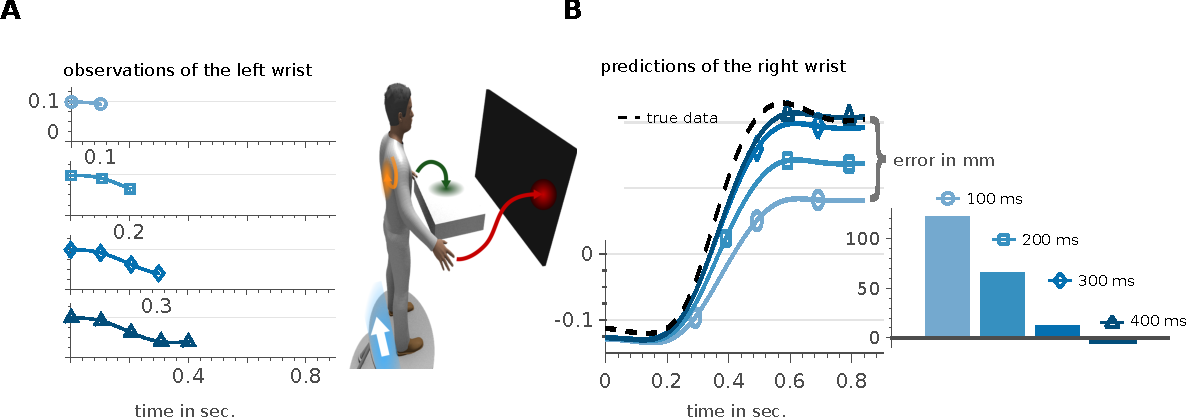
\includegraphics[width=\textwidth]{Elmar/picsClean/Fig3Predictions}
%\label{fig:subfig2}
 \caption{\textbf{Supportive contacts predict goal-directed movements:} 
 \textbf{A)} Partial observations of the left wrist predict right wrist future states in \textbf{B}. 
 For increasing observation horizons of the y-coordinate of the left wrist, 
 the predicted right wrist trajectories converge to the true trajectory (illustrated as dashed line in \textbf{B}). 
 The final Euclidean error (to the true reached target on the screen) of less than $2$ cm after $300$ ms is $40$ times smaller than the distance between the two outer targets (that is $80$ cm). 
}
\label{fig:OpsPrediction}
\end{figure}

For increasing observation horizons up to $400$ ms, exemplary predictions of the 
y-coordinate of the arm trajectories are shown in \FigureAbbr 
\ref{fig:OpsPrediction}. For these examples the target prediction error was 
below $5$ cm when observing only the first $300$ ms of the left wrist motion. 
Note that the distance between the two exterior targets on the screen was $80$ 
cm which defines the maximum error.  Averaged over all subjects, the prediction 
error was $12.3 \, \pm \, 9.8$ cm for an observation horizon of $300$ ms. When 
observing the complete trial the error was $6.4 \, \pm \, 5.5$ cm. Per subject errors are shown in \FigureAbbr 
\ref{fig:subFigPerdErrorAllSubjects}. Note that to obtain these results 
we used $18$ trials for training (trials $170-320$) and $18$ trials for testing (trials $321-400$). %six per target

\begin{figure}[t]
\centering
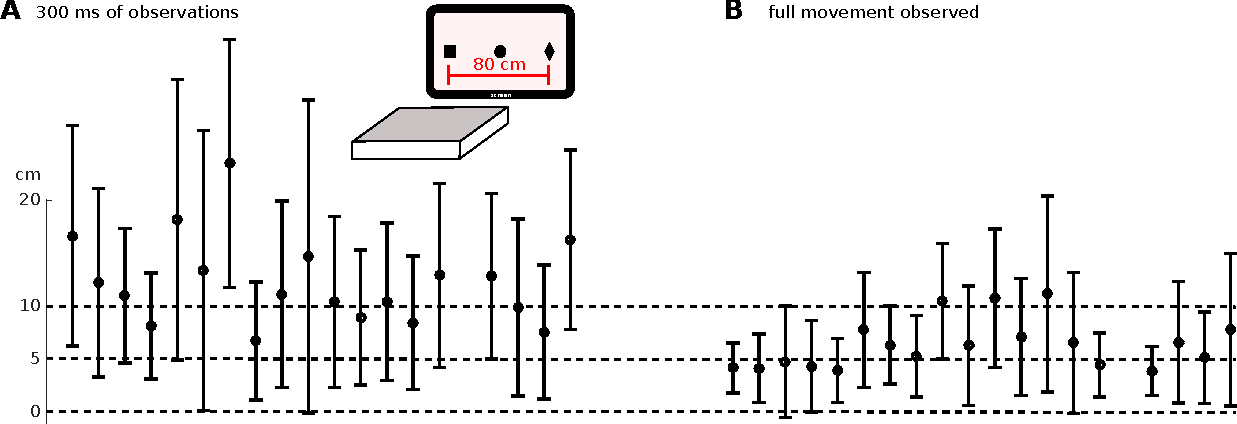
\includegraphics[width=\textwidth]{Elmar/picsClean/SubFigPredError9DoF}
%\label{fig:subfig2}
 \caption{\textbf{Target prediction error over all subjects:} 
 \textbf{A)} Averaged prediction error for $19$ subjects when observing $300$ ms of the left wrist marker trajectories in perturbed trials. 
 \textbf{B)} The prediction error when observing the whole left wrist motion. Illustrated are the mean and the 
 standard deviation over $18$ test trials (six per target). One subject of $20$ was excluded as less than six trials per target were recorded. 
 Note that the maximum error or the distance between the two outer targets in the screen is $80$ cm.
 }
\label{fig:subFigPerdErrorAllSubjects}
\end{figure}

%Conclusion: left wrist can predict the right wrist 
In summary, the PTM was used to train models of trajectory distributions that 
could predict the goal-directed reaching motions from observing solely the 
supportive left wrist movements. Accurate predictions at an early execution 
phase (i.e., the first $300$ ms), where the effect of visual feedback is 
negligible, indicate that supportive contacts are at least partially 
pre-processed. 

%Implication: Supportive contacts predict goal-directed movements

\subsection{Trunk adaptation precedes arm adaptation}

\begin{figure}[t]
\centering
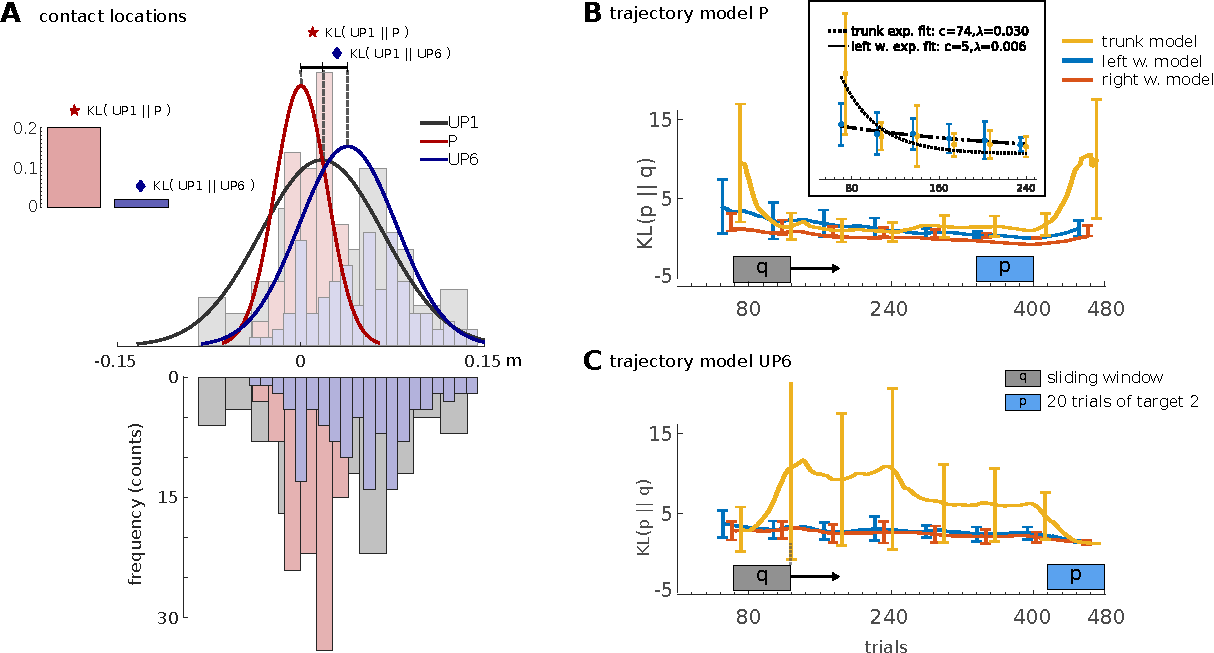
\includegraphics[width=\textwidth]{Elmar/picsClean/Fig4ModelComparison}
%\label{fig:subfig2}
 \caption{\textbf{Trunk adaptation precedes arm adaptation:} 
 \textbf{A)} The adaptation process of the contact location is illustrated by computing the KL-divergence between the first unperturbed session (UP1), the perturbed trials (P), 
 and the last unperturbed session (UP6). The underlying data is shown as histogram with the Gaussian model fits as overlay.
 \textbf{B-C)} For a detailed temporal analysis, the KL-divergence between a set of training trials (a sliding window of 20 trajectories) and 
 a set of test trials (\textbf{B}: last 20 trials in P, \textbf{C}: last 20 trials in UP6) is investigated. 
 An exponential model fit is presented in the inset in \textbf{B}.  
}
\label{fig:OpsModelComparison}
\end{figure}

To investigate adaptation of the supportive contacts we fitted Gaussian 
distributions to the contact locations recorded in the three phases of learning 
--- the unperturbed training phase, the phase of perturbed trials and the final washout phase. 
Histograms over the contact locations in the shoulder frame are shown in \FigureAbbr \ref{fig:OpsModelComparison}A, 
where \textit{UP1} denotes the initial training phase, \textit{P} the perturbed trials and 
\textit{UP6} the sixth session that was the washout phase. During the perturbed trials of the experiment, 
we found a shift of contacts to the right, or in other words, the left hand is moving closer to the 
center of the table in \FigureAbbr \ref{fig:subFigContactLocationsAllSubjects}A 
(Note that the particular values in meters differ in \FigureAbbrP 
\ref{fig:subFigContactLocationsAllSubjects}A and in \FigureAbbrP 
\ref{fig:OpsModelComparison}A. In the later the contacts are plotted in the 
shoulder frame).  

To compare the similarities between the fitted Gaussian distributions for the three phases of 
learning, we used a Kullback-Leibler divergence (KL) distance measure. 
In line with the observation of the shift of contacts, we 
found strong similarities between the unperturbed phases, i.e., KL(UP1$||$UP6) = 
$0.019$. In contrast for the transition to the perturbed trials we computed 
a distance of KL(UP1$||$P) = $0.20$. For the transition to the washout phase, 
we found KL(P$||$UP6) = $0.126$. 
%Note that for these comparisons the last six center targets in each phase of all subjects were used. 


A more detailed investigation was conducted by analyzing trajectory  
similarities using the PTM. As reference model, trajectories of the last $20$ 
trials in P or UP6 were used. We compared the reference model to a trajectory 
model trained from $20$ trials in a moving window. The moving window traverses from trial 
$10$ to trial $460$ which is denoted by the shaded boxes in \FigureAbbrP 
\ref{fig:OpsModelComparison}B and C. 
Individual models were trained for the left wrist, the right wrist and the 
trunk. We found that the trunk model converged about five times faster than the 
left wrist model. For that we used one-term exponential models of the form 
$y\,=\,c\,\exp(\lambda\,x)$, where for the trunk $\lambda_t=0.03$ and for the left wrist $\lambda_l=0.006$. 
This result is highlighted in the inlay in \FigureAbbr \ref{fig:OpsModelComparison}B.
% 
% with $c=74$ and $\lambda=0.03$ for the trunk 
% and $c=5$ and $\lambda=0.006$ for the left wrist. 
% 
% where for the trunk  
% % $c=74$, $\lambda=0.03$ vs. $c=5$, $\lambda=0.006$ for the left wrist where 
% % $0.03/0.006=5$)
% For the trunk the model parameters were $a=74$ and $b=0.03$ compared to . 
% (i.e., exponential fit of the trunk: 
% $c=74$, $\lambda=0.03$ vs. $c=5$, $\lambda=0.006$ for the left wrist where 
% $0.03/0.006=5$), see right column in \FigureAbbr \ref{fig:OpsModelComparison}B. 

We found that the trunk adapts faster than the supportive contact motion. This 
finding can be explained by the importance of correct trunk motions to prevent 
falling as observed in related work \cite{bouisset1981sequence, stapley1999does}. When comparing the prediction accuracy however, we made an interesting 
observation. During early phases of the motor execution the left wrist results 
in more accurate predictions. However, when observing the complete motion, the 
trunk was more informative for predicting the right arm movements, see 
Supplementary \FigureAbbr \ref{fig:SubFigPredErrorTrunkvsLW}. This result 
suggests that the supportive motion has a stronger effect on the task 
performance during early phases compared to the massive trunk. 

%Conclusion: Trunk adaption is more important for the task than wrist movement modifications
%Implication: Evidence for learning on multiple time scales


%DISCUSSION
\section{Discussion}

%controversy: static contacts are known to aid postural control, however it is unknown if they are planned or reactive???
It is known that supportive contacts aid postural control in humans 
\cite{balasubramaniam2002dynamics}. Contacts increase the subjects' belief about 
their poses in board balancing tasks \cite{slijper2000effects}, in tasks without 
visual cues \cite{johannsen2007effects}, and have an effect on learning 
balancing strategies during task adaptation \cite{babivc2014effects}. While 
these studies demonstrated the importance of contacts for human motor control, 
the contacts where \textit{static} and pre-defined based on the experimental 
setting. In this study, we investigated the effect of the \textit{active choice} 
of supportive contacts on motor control. Under natural conditions subjects were 
able to choose supportive contact locations to aid target reaching. Utilizing a 
developed probabilistic trajectory model (PTM), we found that the supportive motions 
leading to contacts could predict goal-directed reaching movements and 
learning proceeds on multiple time scales. These findings have important 
implications on medical care in diseases related to central nervous system 
disorders (such as dementia, Alzheimer's, Parkinson's disease or stroke), 
computational neuroscience and robotics. 

\subsection{A pre-test for central nervous system disorders affecting postural control} 

Many central nervous system disorders affect not only cognitive abilities 
related to memory consolidation but also postural control.  For example, an 
underdevelopment of postural control is a well known symptom in 
autism\cite{schmitz2003motor, minshew2004underdevelopment}. Early detection of 
these diseases is of utter importance for medical care. However, most pre-tests 
focus on cognitive functions that are influenced by many factors such as stress, 
sleep deprivation and age. Classical tests targeting motor coordination 
abilities are unnatural like for example the grooved pegboard 
test\cite{klove1963clinical}, where the goal is to fit pegs of various shapes 
into punched holes. The presented experimental setting has the 
potential to become an alternative pre-test that investigates postural control 
and motor learning under natural conditions. Deficits in motor control can be 
quantified in terms of the model prediction performance as shown in \FigureAbbr 
\ref{fig:OpsPrediction}. In the tested subjects, the average prediction error of the 
goal-directed target reaching motion was $6.4 \, \pm \, 5.5 \textrm{(SD)}$ cm out of a total range of 
$80$ cm. Note that for these predictions the model input was solely the x,y,z coordinate of 
the supportive motion, see \FigureAbbr \ref{fig:subFigPerdErrorAllSubjects}B. 
While the predictions were accurate for the tested healthy subjects, we speculate that 
participants with motor dysfunctions would show inferior prediction performance scores. 

However, a limitation of the presented experimental setting is its simplicity. 
In our experiments the participants reached for a static target at one out of three possible locations  
on a horizontal line. Synchronization of movement onsets within $3-5$ trials (see \FigureAbbr \ref{fig:subFigContactLocationsAllSubjects}C-D) 
indicates that the task might be too simple to show significant effects in subjects 
with central nervous system disorders. More complex tasks could consider for example moving 
targets at arbitrary locations on the screen. 

\subsection{Evidence for learning on multiple time scales}

For many tasks motor memory consolidation proceeds on 
different time scales\cite{wolpert2000computational, 
smith2006interacting, diedrichsen2010coordination}. In particular, postural 
control is adapted on a faster rate in contrast to goal-directed movements. For 
example, Huys et al. showed that postural sway precedes eye and head movements 
($3:2$ or also $3:1$) in subjects learning to juggle\cite{huys2004timescales}. 
In line with this finding, we found that trunk adaptation to maintain balance 
precedes the learning of optimal (here task correlated) supportive contact 
motions. Concretely, the learned trunk model converged about $5$ times faster 
than the left wrist model, see \FigureAbbr \ref{fig:OpsModelComparison}B. This result is 
another indicator for a hierarchical organization of motor control with the 
difference that we analyzed adaptation on a trajectory level in contrast to 
single time step models \cite{kuo1995optimal, wolpert2000computational, 
diedrichsen2010coordination}. The developed PTM  may extend future computational 
models for optimal feedback control by combining sequential predictions of feed 
forward commands and the integration of perceptual feedback. 

A potential deficit of such an optimal feedback controller is that we analyzed 
adaptation on a kinematic level, where limb inertia has a delayed effect on the 
recorded marker trajectories. For example, while expressive motion vectors can 
be observed for the light weight arms, the massive trunk may have moved just for 
few millimeters which could result in inaccurate predictions. This hypothesis is 
confirmed by our results, where at early movement phases (up to $300$ ms) the 
left wrist leads to more accurate predictions than the trunk, see Supplementary 
\FigureAbbr \ref{fig:SubFigPredErrorTrunkvsLW}. For observations of the complete 
trial however, the trunk motion is more informative. To avert the effect of limb 
inertia the PTM could be trained from Electromyography (EMG) patterns. Such 
models could be used to predict motor commands on a muscle level and could help to 
better understand the underlying motor control mechanisms. 

\subsection{A robot controller that actively seeks for contacts}

In this research we studied whole-body coordination mechanisms of arm reaching 
and postural control with additional hand contact. We investigated how humans 
perform reaching movements with the right arm in postural challenged conditions. 
Postural balance was maintained by establishing a supportive hand contact with 
the other arm. In effect, both arms had to perform reaching movements where one 
arm reaches for a distant target and the other arm reaches for a supportive hand 
contact. We found that humans preferred distinct contact locations for each of 
the three targets that were displayed. Such a context dependent controller could 
advance current abilities of humanoid robots as it was envisioned in the 
European project CoDyCo\cite{codyco}. In particular, our results suggest that 
different supportive contact strategies should be initiated based on future intentions. 
This has not been done so far as research on anticipatory controller 
 focused largely on balancing\cite{sugihara2002whole, rueckert2014robust, tassa2012synthesis} or 
 on compensating for external forces\cite{atkeson2007multiple, hyon2007full, ruckert2011study, toussaint2014dual}. 
%Work on contacts focused mainly on following force profiles for manipulation and 
% left postural control relatively unexplored. 

In our experiments the modulating factors (the context) were the distance to the 
target,  its location on the screen and the postural perturbation. The distance 
was chosen such that subjects \textit{always} made a contact to avoid falling 
when reaching. We only investigated the effect of the contact location and used 
pre-defined translateral support base perturbations. The perturbations had no 
effect on the results. In unperturbed and perturbed conditions the subjects 
chose target dependent contact locations, see \FigureAbbr 
\ref{fig:subFigContactLocationsAllSubjects}B. Future research may explore the 
effect of distance to complement a robot controller that autonomously decides in 
which situations to make supportive contacts. 


\section{Methods}%\label{sec:methods}

\subsection{Participants}

Twenty right-handed male subjects ($\textrm{age:} \, 20.8 \, \pm  \, 1.8 \,
\textrm{(SD)}$) participated in the reaching experiments. None reported any neurological or musculoskeletal
disorders (self-reported). Prior to their participation, the subjects were
informed about the course of the study and were required to sign an informed
consent approved by the National Medical Ethics Committee Slovenia (NO. 112/06/13).

\subsection{Apparatus}

Participants stood on a force plate (9281CA, Kistler Instrumente AG, Winterthur,
Switzerland) mounted on top of a Stewart platform \cite{stewart1965platform}.
The force plate was used to measure the six components of the ground reaction
forces and torques to determine the center-of-pressure (CoP). The CoP was only used 
to pre-compute tentative movement onsets (based on two percent peak velocity and CoP criteria).
These pre-computed movement onsets of the left and the right wrist were manually corrected through visual inspection ($480\,\times\,20$ trials). 
% In addition, fluctuations of force component in the superior direction were used
% to improve the movement onset computation based on wrist velocities (see
% Supplementary Fig. X2). 

A second force plate of the same type was mounted anteromedial to the subject's hip
position. This force plate was used like a table providing additional support 
during reaching. The contact locations shown in \FigureAbbr \ref{fig:subFigContactLocationsAllSubjects} were
defined as the left wrist position at the peak supportive contact force. In front to the 
contact force plate we mounted a screen. Both, the force plate and the screen
were adjusted in height based on the subject's trunk height ($56.5 \, \pm \, 2.4$ cm).
%NOTE to JAN: the third marker at the approx. CoM was not used in my code so far

The Stewart platform was used to apply translational perturbations in the 
mediolateral direction. Specifically, the displacement of the platform was 
proportional to the sum of the anteroposterior components of the left and right 
hand displacements. The maximal displacement of the Stewart platform was $20$ cm 
and corresponded to the situation when the subject's left hand was at the far 
edge of the table and the finger on the right hand touched the screen, see 
Supplementary \FigureAbbr \ref{fig:SubFigStewartPert}.

A motion capture system (NDI 3D Investigator) was used to track the participants 
wrists and trunk movements. Three motion tracking markers were attached two each wrist to 
compensate for occlusions during the reaching motions. At least one marker 
needed to be visible and for more than one visible marker the position was 
computed through averaging. Two markers were attached to the back at the 
scapulae to transform wrist trajectories to shoulder frames and to estimate the 
trunk motions (i.e., the center location of the two shoulder markers). 
Additional markers were placed at the screen, at a wearable thimble to estimate 
the right index fingertip position and at the force plate mounted on top of the 
Stewart platform.

\subsection{Coordinate frames}

If not stated different, the results are defined in the subject's coordinate
frame. To compensate for the translational perturbations of the Stewart platform
a marker was attached to the support force plate. The subjects coordinate frame
was defined as the force plate marker position minus the initial left wrist
location (to correct for small deviations of the subject's feet placement
throughout the experiment). 

Wrist trajectories (see \FigureAbbrP \ref{fig:OpsPrediction}) were computed in the shoulder frames to isolate
trunk and arm adaptations. In particular, the wrist positions in the subject's
coordinate frame were additionally corrected by the time-varying shoulder marker positions.  

\subsection{Procedure}

Participants had to perform $480$ trials of reaching in blocks of $80$ trials.
After each block the subjects had a five minutes break. Only the first and the
last $80$ trials were unperturbed (see \FigureAbbrP 
\ref{fig:subFigContactLocationsAllSubjects}b). To investigate
negative after effects, the perturbation was deactivated for $30$ randomly selected reachings  
during trials $240$ to $400$. The participants were not informed about these
catch trials. 
%5     9    14    19    22    26    32    36    41    47    51    57    64    69     73    79

Prior to each trial, subjects were required to stand upright moving as little as
possible. A bar on the screen indicated anteroposterior fluctuations of the CoP
in real time with respect to the initial CoP value. This initial CoP was measured at the beginning of
the experiment. If the mean of the deviations averaged over $500$ ms was less
than $1$ cm the start of the trial was initiated. After one second the target
was presented at one out of three locations (target onset). After a random
period ($1-3$ sec) the target's color switched and the subjects were allowed to
move. Movements prior to that visual cue terminated the trial. The target was
reached if the distance between the fingertip and the target on the screen was
less than $1$ cm. 

Participants received a monetary reward after each trial based on the time
needed for reaching, i.e., $\textrm{EUR}\,=\,0.1 \, - \, 0.05 \, t\,$ where $t$ denotes the reaching time in seconds. 
The reaching time was defined as the difference between the target onset and the time until the target
was reached. On average the subjects received five cents per trial which corresponds to a reaching duration of one second, see Supplementary \FigureAbbr \ref{fig:SubFigRewards}. %On average our subjects earned $20X \, \pm \, xx$ EUR.
 If the target was missed, or if the target was not reached within
two seconds, no reward was given. 

\subsection{Data processing}

All measurements of the force plates and the motion capture system were recorded at a rate of $100$ Hz. Redundant marker settings on the
wrists and on the thimble were used to compensate for occlusions. For that three markers were used 
for both wrists and the thimble. If all markers were occluded the trial was excluded from the analysis. 
For two or three correctly observed markers we computed the average for each coordinate (x,y,z). 
All marker trajectories were low-pass filtered at $5$ Hz using $2$nd-order Butterworth filter.
% Fs = 100; %100Hz
%     Fc = 5; %Hz
%     order = 2;
%     [f, e] = butter(order, Fc*2/Fs, 'low');


\subsection{Statistical tests}

Statistical analyses were performed using SPSS 21 (SPSS Inc., Chicago, USA). For 
each subject, an average of left hand contact location in mediolateral direction 
was calculated for every combination of balance perturbation (unperturbed, 
perturbed and unperturbed catch trials) and target locations. The average values 
of the individual subjects were then used for statistical analysis. Effect of 
perturbation was investigated using one-way repeated measures ANOVA. Differences 
between perturbed and unperturbed sessions for each combination of independent 
variables were tested with post hoc t-tests with Bonferroni correction. The 
level of statistical significance was set to $0.05$.
    
\subsection{Computing predictions through conditioning}
%
Conditional probabilities and predictions are related concepts in statistical
modeling. A prediction problem can modeled as computing the conditional
probability denoted by 
\begin{equation}
p(B \, | \, A) = p(A,B) \, / \, p(A) ~~, \label{eq:cond_prob}
\end{equation}
where $A$ and
$B$ represent two random variables (RVs). In our experiment, the variable $A$
could encode the probability of a certain contact location on the table and the
target location is represented by the RV $B$. The joint distribution $p(A,B)$ is
the learned model and $p(A)$ is a prior over all possible contact locations.
Given a particular contact location $p(A=a)$, we can compute the most likely 
target the human tries to reach. Throughout the paper, we will use the shorthand
$p(a)$ to denote $p(A=a)$, which is the probability that the RV $A$ takes the
value $a$ to keep the notation uncluttered. 

A particular interesting class of distributions are Gaussian distributions 
\begin{equation}\label{eq:gaussian}
 N(\vec x \, | \, \vec \mu, \vec \Sigma) \coloneqq \frac{1}{{(2\pi)}^{n/2} \, \sqrt{\textrm{det} \vec \Sigma}} \, 
    \exp \left( -\frac{1}{2} (\vec x - \vec \mu)^T \, \vec \Sigma^{-1} \, (\vec x - \vec \mu) \right) ~~,
\end{equation}
 with the $n$-dimensional RV $\vec x \in \mathbb{R}^n$, the mean $\vec \mu$ and the variance $\vec \Sigma$. 
%, i.e. $\N(x | \mu, \Sigma)$ with the RV $x$, mean $\mu$ and variance $\Sigma$. 
In Gaussian distributions, conditional distributions can be computed in closed form. To see
this, we define a multivariate normal distribution by concatenating two RVs. The two RVs denote the contact locations and the targets, i.e., $\vec x = {a \choose b}$, $\vec \mu =
{\mu_a \choose \mu_b}$ and $\vec \Sigma = \left( \begin{smallmatrix}
\Sigma_{aa}&\Sigma_{ab}\\ \Sigma_{ba}&\Sigma{bb} \end{smallmatrix} \right)$. 
Using these definitions  
in \eqref{eq:gaussian} and after rearranging the terms, the
parameters $\mu_{b|a}$ and $\Sigma_{b|a}$ of the conditional distribution can be computed as 
\begin{eqnarray}\label{eq:general_cond_param}
  p(b \, | \, a) \;&=&\; \N(b \, | \, \mu_{b|a},\Sigma_{b|a}) ~~, \\
   & \text{with} & ~~~ \mu_{b|a}  =  \mu_b + \Sigma_{ba} {\Sigma_{bb}}^{-1} (a - \mu_a) ~~, \nonumber\\
  & \text{and} & ~~~ \Sigma_{b|a} = \Sigma_{bb} - \Sigma_{ba}{\Sigma_{bb}}^{-1}\Sigma_{ab}  ~~. \nonumber
\end{eqnarray}
Given multiple measurements of $a$ and $b$ we can compute the statistics $\vec \mu$ and
$\vec \Sigma$. For some during training unseen contact location $a^*$ we can now
predict the most likely target location (parametrized through $\mu_{b|a^*}$ and
$\Sigma_{b|a^*}$). In the following we will extend this powerful feature of computing predictions to time-series data or trajectories. 

\subsection{Phase modulated probabilistic models of trajectories}
%minimal description, details are given in Box 1
The same conditioning operation can be used for computing predictions in trajectories if the RVs 
encode feature vectors in function approximation, see \FigureAbbr \ref{fig:model} for a sketch. 
Let $\vec y_t = {a_t \choose b_t}$ denote a concatenated state at time $t$ representing the contact location and the target. 
Only for the sake of clarity we will again assume that the contact location and the target are 
scalars. As we will see later the results generalize to multi-dimensional states. 
In addition, we will assume for simplicity that each dimension in $\vec y_t$ is 
approximated through a $J$-dimensional feature vector $\vec w \in \mathbb{R}^{J \times 1}$ 
and basis function vectors $\vec \phi_t \in \mathbb{R}^{1 \times J}$, 
e.g.  $a_t = \vec \phi_t \, \vec w_a$ with $\vec \phi_t = \left[\phi_{t,1},\, ..., \, \phi_{t,J}\right]^T$. 
A large variety of possible basis functions can be used for time series approximation. A popular choice 
for rhythmic movements are Von-Mises basis functions, 
whereas Gaussian basis functions are widely used for point to point movements \cite{Rueckert2013, ijspeert2013dynamical} 
\begin{equation*}
 \phi_{t,i} = \frac{1}{\mathcal{Z}} \, \exp \left( -\frac{1}{2 h} \left(z(t) - c_i \right)^2 \right) ~~,
\end{equation*}
where $\mathcal{Z} = \sum_{l=1}^J \exp \left( -1\,/\,2 h \left(z(t) - c_l \right)^2 \right)$ denotes a normalization term.  
The function $z(t)$ implements a mapping from discrete time steps to a movement phase, i.e., $z: t \in [1,T] \mapsto [0,1]$. 
In this notation state sequences of different length can be modeled and are aligned through the movement phase. 
Note that in our reaching experiments $z(t)=0$ denotes the movement onset and $z(t)=1$ the event when the target was reached. 
The scalar $c_i \in [0,1]$ denotes the center of the $i$-th basis function and $h$ is the bandwidth 
parameter. 

In general, $D$-dimensional states can be approximated in $\vec y_t = \vec
\Phi_t \; \vec w$ using block diagonal matrices $\vec \Phi_t \in \mathbb{R}^{D
\times J D}$ and concatenated feature vectors $\vec w = \left[w_1^T,\, ...,\,
w_D^T\right]^T \in \mathbb{R}^{J D \times 1}$. For example, when modeling
contacts and targets,  $\vec w = \left[w_a^T, w_b^T\right]^T$ and a block
diagonal matrix of the form $\vec \Phi_t = \left( \begin{smallmatrix} \vec
\phi_t & \vec 0 \\ \vec 0 & \vec \phi_t \end{smallmatrix} \right)$ is used. 

Sequences of $T$ states, denoted by $\vec \tau = \vec y_{1:T}$, can be compactly represented by 
\begin{eqnarray}
    \vec \tau \;=\; \vec \Phi_{1:T} \, \vec w ~~~~ 
    \text{with} ~~~~ \vec \Phi_{1:T} = \left[\vec \Phi_1^T,\, ...,\, \vec \Phi_T^T\right]^T \in \mathbb{R}^{T D \times J D} ~~,  \label{eq:func_approx_general} 
\end{eqnarray}
where $\vec \Phi_{1:T}$ denotes an extended basis function matrix. 
Using the function approximation in \eqref{eq:func_approx_general} we can define the 
generative probabilistic model for trajectories 
\begin{equation*}
p(\vec \tau \, | \, \vec w) = \prod_{t=1}^T \N\left(\vec y_t \middle| \vec \Phi_{t} \, \vec w, \vec \Sigma_y \right)  \; = \; \N\left(\vec y_{1:T} \middle| \vec \Phi_{1:T} \, \vec w, \vec \Sigma_y \right) ~~,   
\end{equation*}
where $\vec \Sigma_y$ models zero mean independent and identically distributed (i.i.d.) Gaussian noise in $\vec y_t = \vec \Phi_t \; \vec w + \vec \epsilon_y$ 
with $\vec \epsilon_y \sim \N\left(\vec \epsilon_y \, | \, \vec 0, \vec \Sigma_y \right)$. 
%
In order to represent a distribution over trajectories $p(\vec \tau)$, 
we can apply the product rule shown in \eqref{eq:cond_prob} and compute the marginal. 
For Gaussian distributions, in particular for $p(\vec w) = \N\left(\vec w\middle| \vec \mu_w, \vec \Sigma_w \right)$, 
the marginal can be computed in closed form 
\begin{eqnarray}
  p(\vec \tau) &=&  \int p(\vec \tau \, | \, \vec w) p(\vec w) d\vec w \nonumber \\
    &=&  \int \N\left(\vec y_{1:T} \, | \,  \vec \Phi_{1:T} \, \vec w, \vec \Sigma_y\right)  \N\left(\vec w \, | \, \vec \mu_w, \vec \Sigma_w\right) d\vec w \nonumber \\
    &=& \N\left(\vec y_{1:T} \, | \, \vec \Phi_{1:T} \, \vec w,\; \vec \Phi_{1:T} \, 
      \vec \Sigma_w \, \vec \Phi_{1:T}^T + \vec \Sigma_y\right) ~~. \label{eq:feature_to_traj}
\end{eqnarray}
The mean $\vec \mu_w$ 
and the covariance matrix $\vec \Sigma_w$ can be learned from data by maximum likelihood using the Expectation Maximization (EM) algorithm \cite{Dempster1977}. 
A simpler solution that works well in practice is to compute first the most likely estimate of $\vec w^{[i]}$ for each trajectory $\vec \tau^{[i]}$ independently,  
where the index $i$ denotes the $i$-th demonstration.   
In particular, given the trajectory $\vec \tau^{[i]}$, the corresponding 
weight vector $\vec w^{[i]}$ can be estimated by a straight forward least squares estimate
\begin{equation}
 \vec w^{[i]} = \left(\vec \Phi_{1:T}^T \, \vec \Phi_{1:T} + \lambda \, \vec I\right)^{-1} \, \vec \Phi_{1:T}^T \; \vec \tau^{[i]} ~~. \label{eq:lin_reg_traj}
\end{equation}
Subsequently, the mean and the covariance of $p(\vec w)$ can be estimated 
by the sample mean and sample covariance of the $\vec w^{[i]}\,$ vectors. 

\subsection{Computing predictions in trajectories}
%partial spatio-temporal observations encoded in o, \Phi_o and \Sigma_o
Let us assume that we have observed a sequence of states $\vec y_{t_1}$ to $\vec y_{t_M}$ at $m=1,2, ..., M$ different time points, 
which do not need to be sampled at uniform intervals. In addition, not all of the dimensions in the vector 
$\vec y_{t_m}$ might be observed (e.g. due to occlusions, where irrelevant dimensions are assumed to be set to some real number). 
We introduce the homogeneous covariance matrix $\boldsymbol{\Sigma}_{\vec o}$ to control the importance of the observations, 
where small diagonal variances denote important dimensions and large scalars irrelevant dimensions. 
For example, we would use $\boldsymbol{\Sigma}_{\vec o} = \left( \begin{smallmatrix} 1e-5&0\\ 0&1e5 \end{smallmatrix} \right)$ 
if only the first out of two dimensions is observed (as in the example with contact locations and targets). 
Let us further denote $\vec \Phi_{\vec o}$ as the concatenation of the basis function matrices for these time points 
and $\vec o$ as concatenation of the $\vec y_{t_m}$ vectors. 
Given these observations, we can obtain a conditioned distribution $p(\vec w| \vec o)$ over the weight vectors 
%conditioning result
\begin{eqnarray*}
    p(\vec w_o \, | \, \vec o) \;& \propto &\; \N(\vec o \, | \, \vec \Phi_{\vec o} \, \vec w_o, \boldsymbol{\Sigma}_{\vec o}) \, p(\vec w) ~~ \\
     \;& \coloneqq &\; \N(\vec w_o \, | \, \boldsymbol{\mu}_{\vec w| \vec o}, \boldsymbol{\Sigma}_{\vec w|\vec o}) ~~, \\
    & \text{with} & ~~~ \boldsymbol{\mu}_{\vec w| \vec o}  =  \boldsymbol{\mu}_{\vec w} + 
      \boldsymbol{\Sigma}_{\vec w}\boldsymbol{\Phi}_{\vec o}^T\left(\boldsymbol{\Sigma}_o + 
      \boldsymbol{\Phi}_{\vec o}\boldsymbol{\Sigma}_{\vec w}\boldsymbol{\Phi}_{\vec o}^T\right)^{-1}\left(\vec o -\boldsymbol{\Phi}_{o}\boldsymbol{\mu}_{\vec w}\right) ~~,  \\
    & \text{and} & ~~~ \boldsymbol{\Sigma}_{\vec w|\vec o} =  \boldsymbol{\Sigma}_{\vec w}-
      \boldsymbol{\Sigma}_{\vec w}\boldsymbol{\Phi}_{\vec o}^T\left(\boldsymbol{\Sigma}_o 
      +\boldsymbol{\Phi}_{\vec o}\boldsymbol{\Sigma}_{\vec w}\boldsymbol{\Phi}_{\vec o}^T\right)^{-1}\boldsymbol{\Phi}_{\vec o} \boldsymbol{\Sigma}_{\vec w} ~~, 
\end{eqnarray*}
which recovers the conditioning result in \eqref{eq:general_cond_param} in the feature space. 
%prediction result

To predict the state sequence $\vec{\tilde{y}_{1:T}}$, the 
conditional distribution is projected back into the trajectory space using \eqref{eq:feature_to_traj}. 
The result is a distribution over trajectories %Our goal is to predict future states $\vec \tilde{y}_1:T$ given the observations $\vec o$. 
\begin{eqnarray}
  p(\vec \tilde{\tau}) = \N\left(\vec{\tilde{y}_{1:T}} \, \middle| \, \vec \Phi_{1:T} \, \boldsymbol{\mu}_{\vec w| \vec o} \, , \, \vec \Phi_{1:T} \, 
		  \boldsymbol{\Sigma}_{\vec w|\vec o} \, \vec \Phi_{1:T}^T + \vec \Sigma_y\right) ~~, \label{eq:cond_prob_traj}
\end{eqnarray}
where for $t_M < T$ in the observations $\vec o = [\vec y_{t_1}, \vec y_{t_2}, \dots, \vec y_{t_M}]$ future states can be predicted.

\subsection{Computing model comparisons in trajectories}

Using the proposed probabilistic trajectory model (PTM), two trajectory models can be compared through computing the Kullback-Leibler (KL) divergence. 
For Gaussian distributions as in \eqref{eq:feature_to_traj} the KL divergence can be computed in closed form 
\begin{eqnarray*}
 \textrm{KL}(\N_1 || \N_2) = \frac{1}{2} \, { \log \, \frac{ |\vec{\Sigma_2}| }{ |\vec{\Sigma_1}| } \, - n \, + \textrm{tr}({\vec{\Sigma_2}}^{-1} \vec{\Sigma_1}) 
 + (\vec{\mu_2} - \vec{\mu_1})^T \, {\vec{\Sigma_2}}^{-1} \,  (\vec{\mu_2} - \vec{\mu_1}) 
 \, } ~~,  
\end{eqnarray*}
where $\N_1$ denotes a Gaussian with the $n$-dimensional mean $\vec{\mu_1}$ and the covariance $\vec{\Sigma_1}$. The symbol $\textrm{tr}$ denotes the matrix trace. 

\subsection{Computing task likelihoods in trajectories}

Another important probabilistic operation is the computation of the task likelihood. 
This operation can be used to test which candidate model out of several best explains the data. 
Let $\N_p(\, . \, | \, \vec{\mu}, \, \vec{\Sigma})$ denote the model under test. 
Given a single trajectory sample $\vec \tau^*$ and its feature space representation $\vec w^*$ we can compute  
\begin{eqnarray*}
 \textrm{L}(\vec w^* | \N_p) &=& \log \, \N_p(\vec w^* \, | \, \vec{\mu}, \vec{\Sigma} ) \\ 
 &=& - \frac{1}{2} (\vec{\mu} - \vec w^*)^T \, {\vec{\Sigma}}^{-1} \,  (\vec{\mu} - \vec w^*) \, + \, \textrm{a constant} ~~,  
\end{eqnarray*}
which quantifies how likely $\vec \tau^* = \vec \Phi_{1:T} \, \vec w^*$  was generated by model $\N_p(\, . \, | \, \vec{\mu}, \, \vec{\Sigma})$. 


%\renewcommand{\thesection}{S\arabic{section}}  
%\renewcommand{\thetable}{S\arabic{table}}  
%\renewcommand{\thefigure}{S\arabic{figure}} 
%\renewcommand{\theequation}{S\arabic{equation}} 

\section{Supporting Information}

\begin{figure}
\centering
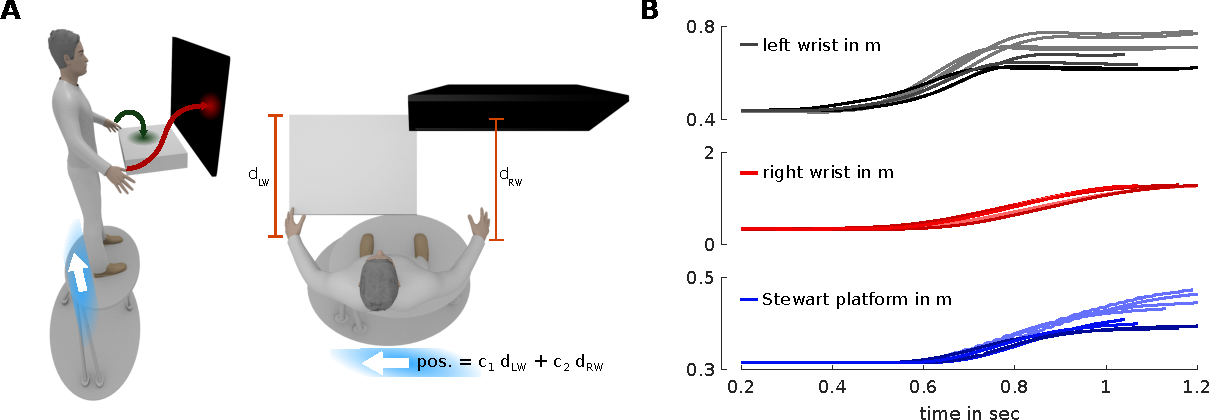
\includegraphics[width=\textwidth]{Elmar/picsSupp/SubFigStewartPert}
%\label{fig:subfig2}
 \caption{\textbf{Supplementary figure, Translateral perturbations:} 
 \textbf{A)} The Stewart platform was used to apply translational perturbations in the mediolateral direction. Specifically, the displacement of the platform was proportional to the sum of the anteroposterior components of the left and right hand displacements. This is denoted by $d_{\textrm{LW}}$ and $d_{\textrm{RW}}$ with the constants $c_1$ and $c_2$. The maximal displacement of the Stewart platform was $20$ cm and corresponded to the situation when the subject's left hand was at the far edge of the table and the finger on the right hand touched the screen. \textbf{B)} Sample trajectories of the left wrist, the right wrist and the displacement of the platform. 
 }
\label{fig:SubFigStewartPert}
\end{figure}


\begin{figure}
\centering
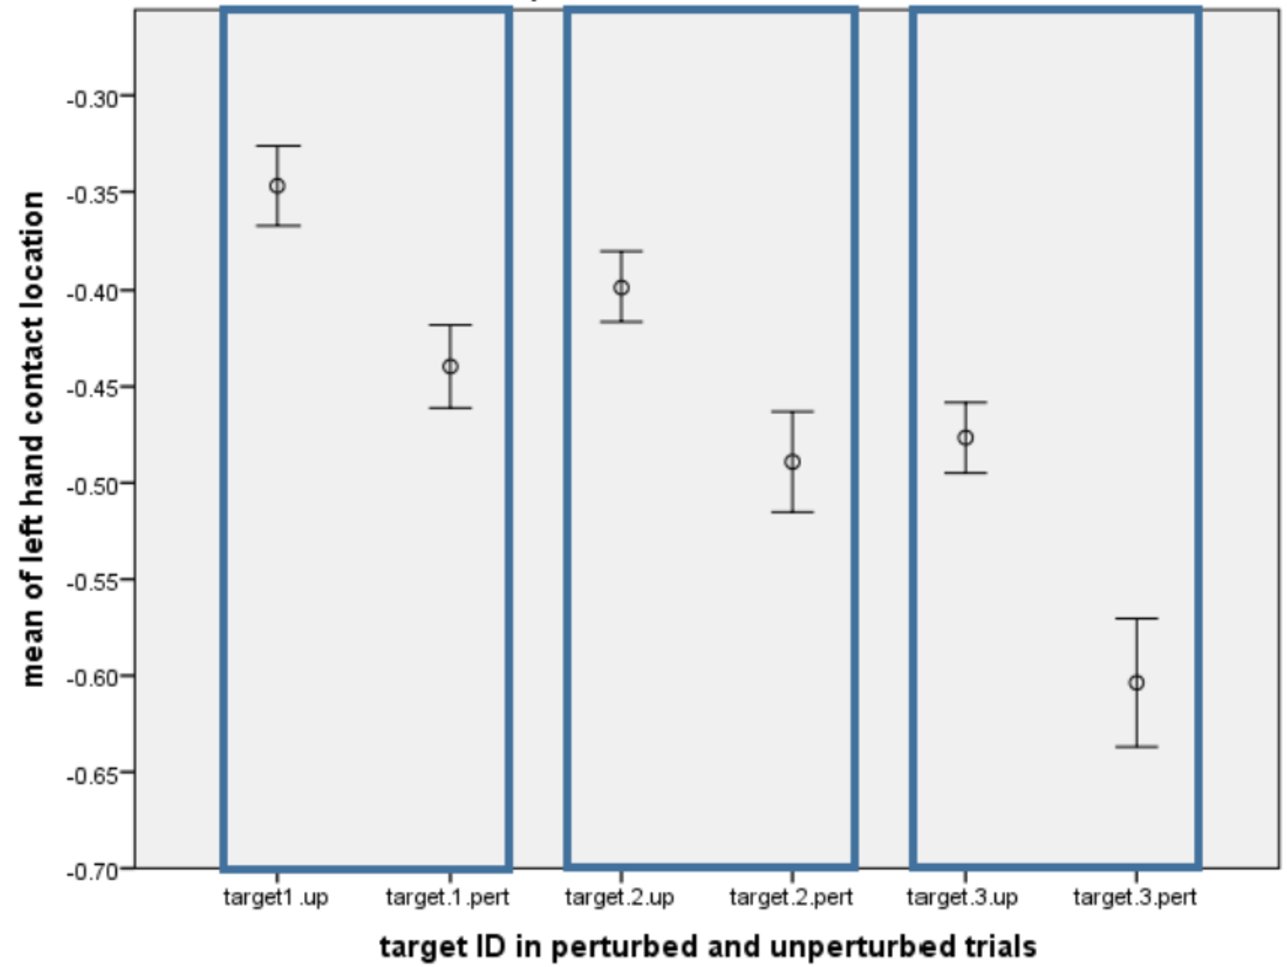
\includegraphics[width=.7\textwidth]{Elmar/picsSupp/SubFigANOVAContactsUPvsPNoTitle}
%\label{fig:subfig2}
 \caption{\textbf{Supplementary figure, Means of the contact locations:} 
 From left to right the means are shown for the three target locations, where we contrast in each panel the unperturbed and the perturbed session.  
 }
\label{fig:SubFigANOVAContacts}
\end{figure}



% \begin{figure}
% \centering
% 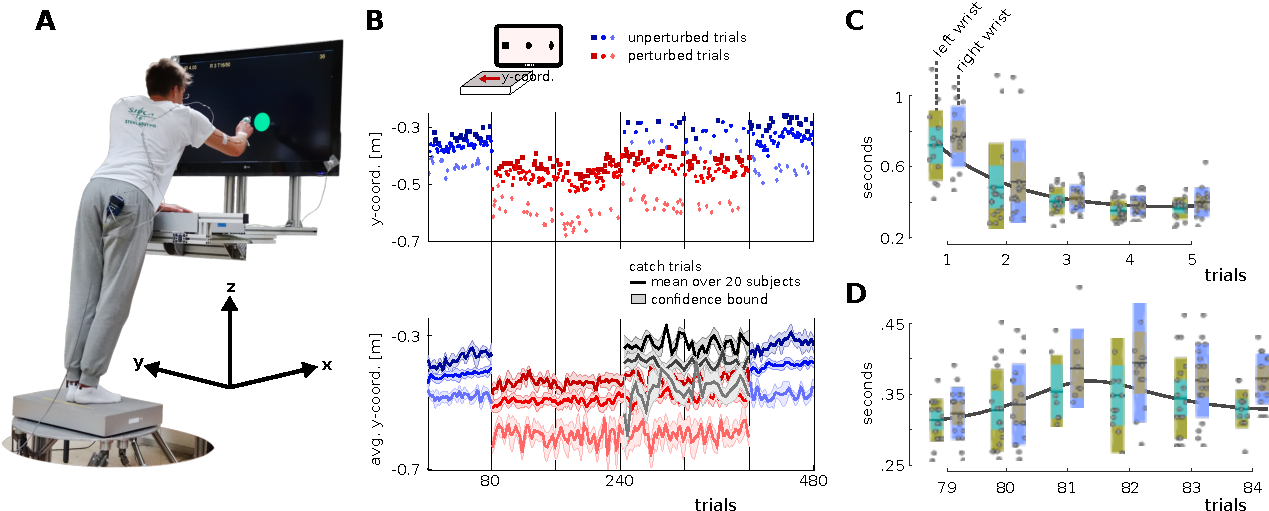
\includegraphics[width=\textwidth]{Elmar/picsClean/Fig1ExperimentContactsOnsets}
% %\label{fig:subfig2}
%  \caption{\textbf{Experiment and Adaptation:} (a) Experimental setting. 
%  (b) The top row shows contact locations for a single representative subject 
%  and the bottom row shows the mean and the confidence bound over all $20$ subjects. 
%  The first $80$ trials and the last $80$ trials ($400$ to $480$) are unperturbed sessions. 
%  Catch trials were initiated during trials $240$ to $400$. Note that during catch trials the contact 
%  location immediately switches back to the unperturbed behavior. This can be explained by the fact that the contact location 
%  is a result of both, the trunk motion (which shows strong negative after effects) and the left wrist motion (were we could not find these effects). 
%  Another finding is that contact locations are target correlated denoted by the three lines in (b). 
%  (c) Illustration of the movement onsets of the wrists for the first five trials (top row) and for the trials transitioning to the first perturbed session (bottom row). 
% }
% %\label{fig:subFigContactLocationsAllSubjects}
% \end{figure}


\begin{figure}
\centering
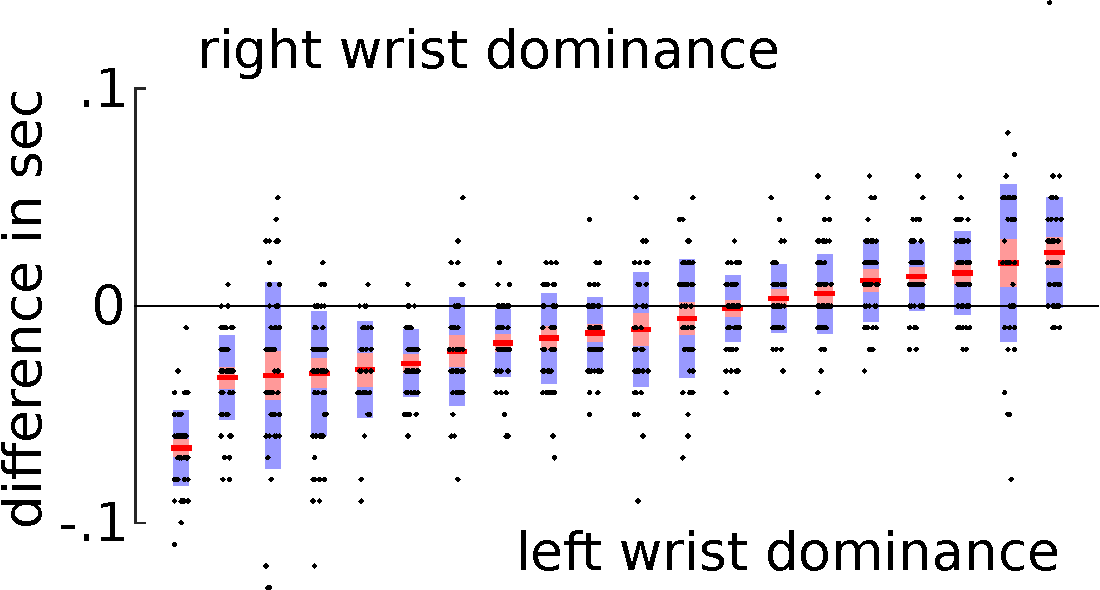
\includegraphics[width=.6\textwidth]{Elmar/picsSupp/SubFigWristPriorities}
%\label{fig:subfig2}
 \caption{\textbf{Supplementary figure, Dominance of the left wrist in 12 out of 20 subjects:} We show the difference of the movement onsets (left wrist minus right wrist). 
 The underlying data are representative trials of the $2$nd perturbed session ($170$ to $240$), where learning converged. The movement onsets were manually corrected through visual inspection. 
 }
\label{fig:subFigWristPriorities}
\end{figure}

% \begin{figure}
% \centering
% 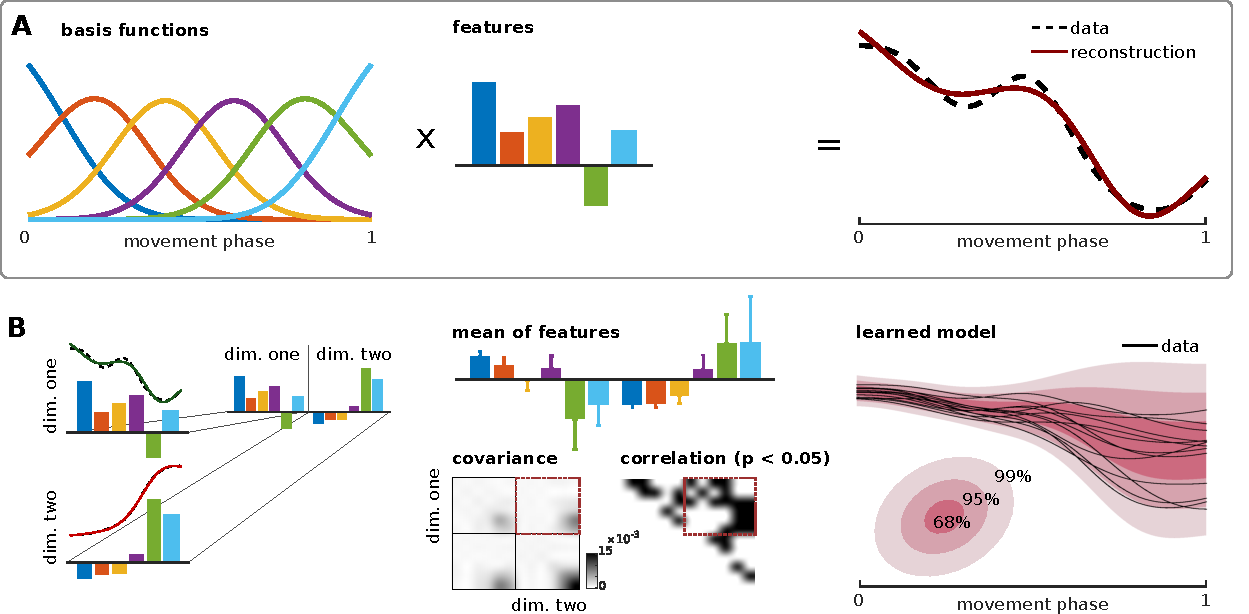
\includegraphics[width=1\textwidth]{Elmar/picsClean/AProbModelofMotionApproach1}
% %\label{fig:subfig2}
%  \caption{\textbf{Probabilistic model of trajectories, from a feature space (left column) to trajectories (right column):}  
%  (a) Generative model. 
%  Equally spaced (radial) basis functions are amplitude scaled by a feature vector to approximate a one-dimensional trajectory. 
%  A movement phase substitutes time to model trajectories of different lengths. 
%  In the inverse direction, feature vectors are computed given the input trajectories using, e.g., standard linear regression techniques or 
%  iterative variational approaches like expectation-maximization. 
%  (b) Learning the correlations between multi-dimensional input trajectories. 
%  Feature vectors computed from multiple input trajectories are concatenated 
%  and the mean and the covariance are computed from multiple trials (or subjects). 
%  The learned correlation is the key features for computing predictions from 
%  partial observations or different input dimensions than the predicted one (e.g., predicting the right wrist trajectory given the left wrist traj. in reaching). 
% }
% \label{fig:model}
% \end{figure}

\begin{figure}
\centering
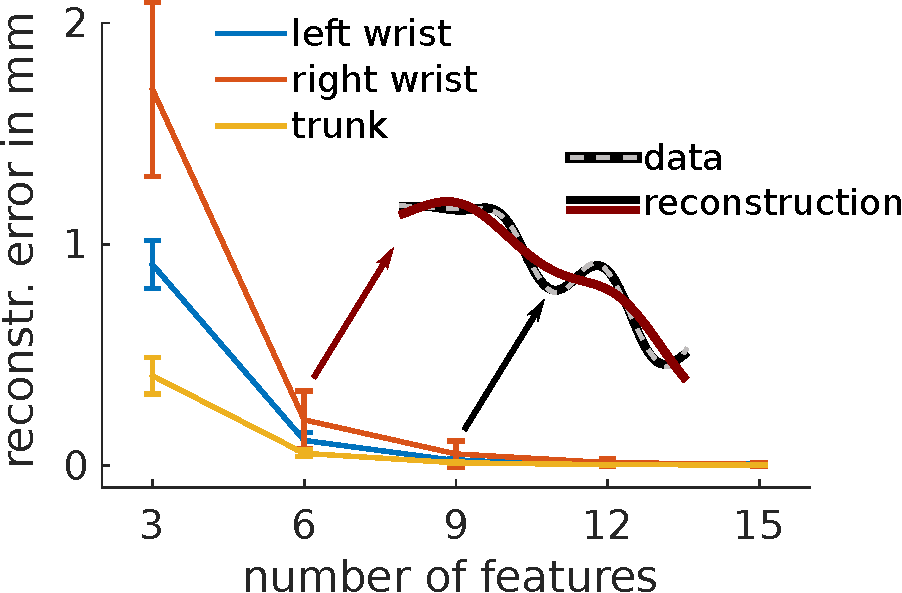
\includegraphics[width=.5\textwidth]{Elmar/picsSupp/NumGaussianFeatures}
%\label{fig:subfig2}
 \caption{\textbf{Supplementary figure. Model complexity (number of basis functions) determines the reconstruction error:}  
 With an increasing number of basis functions the reconstruction error (shown in millimeter) decreases. 
 The reconstruction error is defined as the Euclidean distance of the generated trajectory to its observed counterpart. 
 For the three limbs, left wrist, right wrist and trunk, the error converges to zero with more than nine basis functions. 
 Ten basis functions are used in the experiments in the manuscript. 
}
\label{fig:subFigNumGaussians}
\end{figure}

% \begin{figure}
% \centering
% 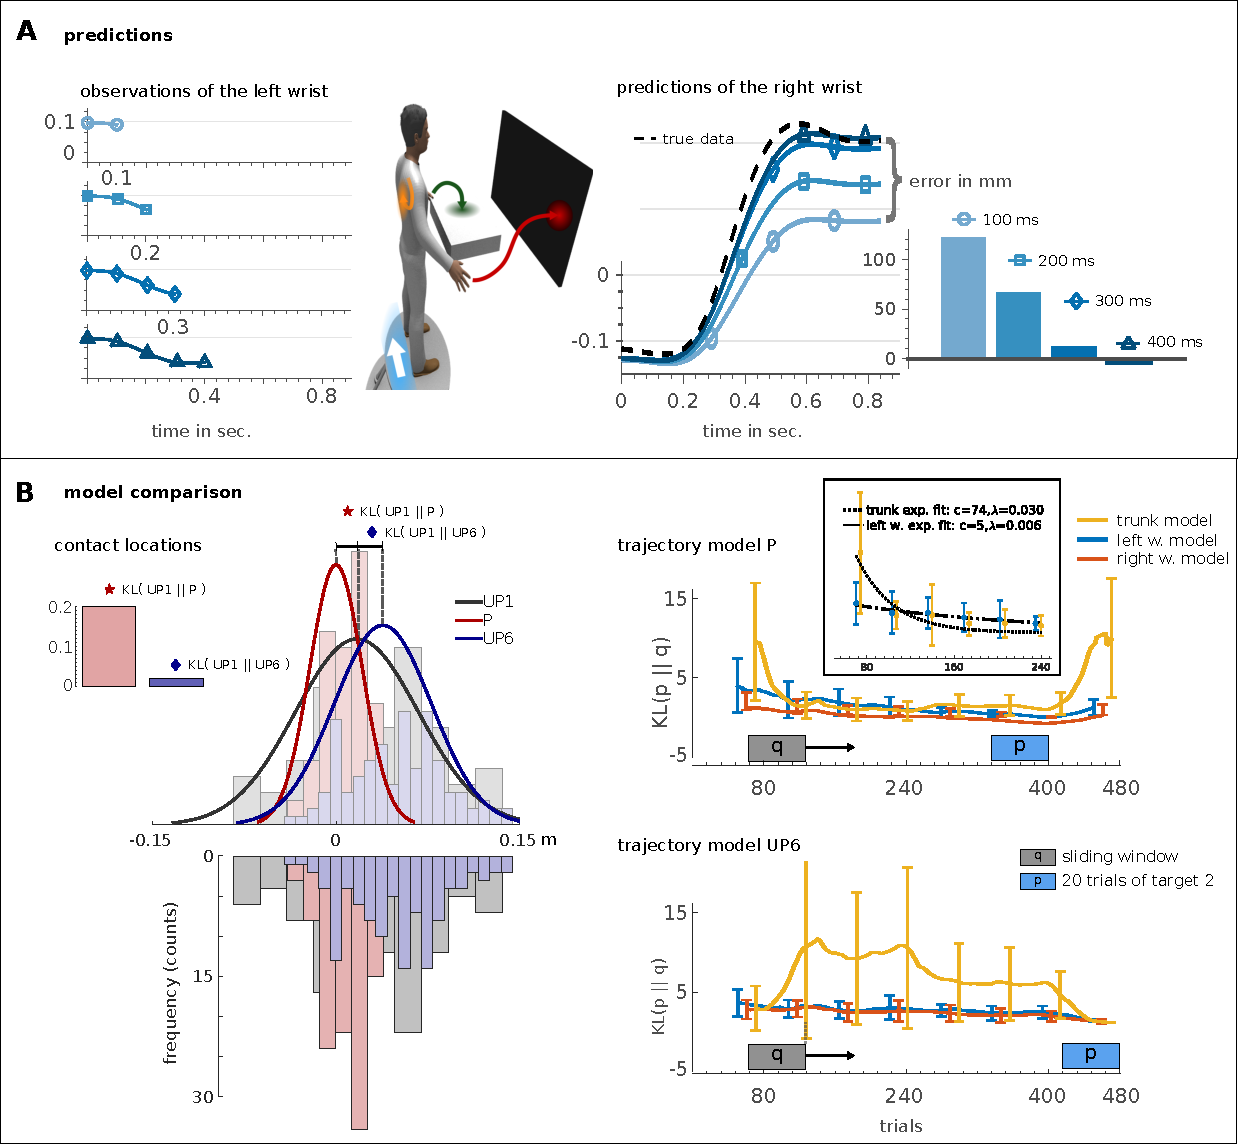
\includegraphics[width=\textwidth]{Elmar/picsClean/FigProbOpsPart1of3}
% %\label{fig:subfig2}
%  \caption{\textbf{Probabilistic operations, predictions and model comparison:} 
%  (a) Partial observations of the left wrist predict right wrist future states. 
%  For increasing observation horizons of the y-coordinate of the left wrist, 
%  the predicted right wrist trajectories converge to the true trajectory (illustrated as dashed line in the right panel). 
%  The final Euclidean error (to the true reached target on the screen) of less than $2$ cm after $300$ ms is $40$ times smaller than the distance between the two outer targets (i.e., $80$ cm). 
%  (b) Perturbations induce adaptation which can be characterized by means of the Kullback-Leibler (KL) divergence. 
%  The left column shows results for the contact location at three stages of learning, 
%  whereas the right panel computes model changes on a trajectory basis and provides a fine temporal resolution. 
%  The adaptation process of the contact location is illustrated by computing the KL-divergence between the first unperturbed session (UP1), the last perturbed session (P), 
%  and the last unperturbed session (UP6). The underlying data is shown as histogram with the Gaussian model fits as overlay.
%  For a detailed temporal analysis, the KL-divergence between a set of training trials (a sliding window of 20 trajectories) and 
%  a set of test trials (top row: last 20 trials in P, bottom row: last 20 trials in UP6) is investigated. 
%  An exponential model fit is presented in the inset.  
%  %only target 2 in the center of the screen
% }
% \label{fig:probOps1}
% \end{figure}

%\begin{figure}
%\centering
%\includegraphics[width=\textwidth]{pics/FigProbOpsPart2of3}
%%\label{fig:subfig2}
% \caption{\textbf{Probabilistic operations, catch trial log likelihood:} 
% Negative after effects (when the perturbation is unexpectedly deactivated) typically result 
% in an overcompensation visible for trunk trajectories 
% but not for left wrist trajectories (denoted by $d$ and shown in the left column for a representative subject). 
% The top row shows results for trunk trajectories and the bottom row for left wrist trajectories. 
% The amount of overshooting (denoted by the distance $d$) depends on the observation horizon 
% and can even be zero if all trajectories converge to the same end-point. Thus a clear statement is often not possible.  
% The probabilistic model approach provides an alternative measure, which is the (log) likelihood that the catch trials 
% was generated by a particular model. In the reaching experiment, we contrast the models of the unperturbed session one (UP1) 
% and the last perturbed session (P). 
% Although that the catch trials were initiated during session P, P is less likely the generative model than UP1. 
% In fact the true generative model is unknown, however, we can conclude that the catch trial is more similar to trials in UP1 than in P which 
% suggests a negative after effect. For the left wrist trajectories no change in behavior is visible in the log likelihood (bottom row in the center column). 
% Results for all subjects are shown in the right column and elucidate that the results in the center column is representative for all subjects.
%}
%\label{fig:probOps2}
%\end{figure}

% \begin{figure}
% \centering
% 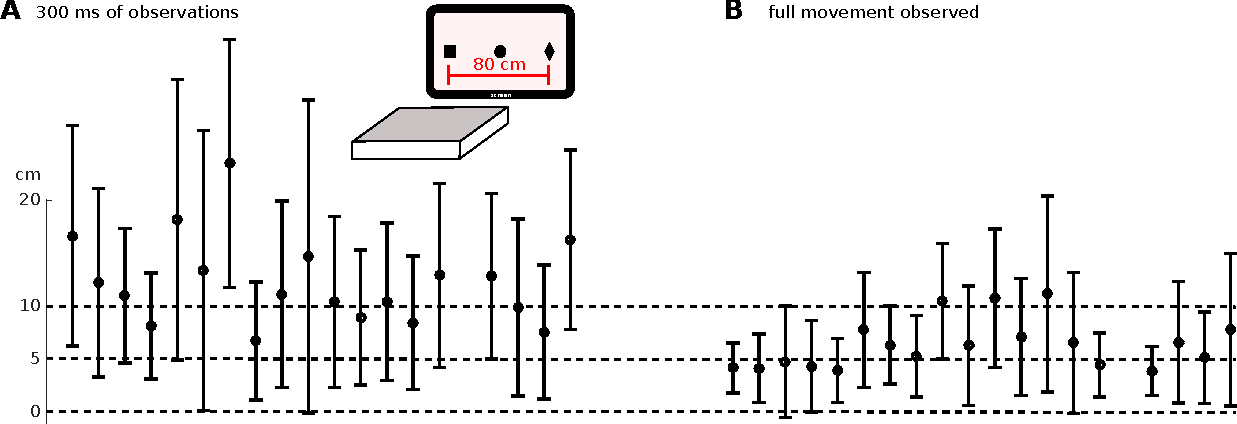
\includegraphics[width=\textwidth]{Elmar/picsClean/SubFigPredError9DoF}
% %\label{fig:subfig2}
%  \caption{\textbf{Supplementary figure, Target prediction error:} 
%  The left panel shows the averaged prediction error for $19$ subjects when observing $300$ ms of the left wrist marker trajectories in perturbed trials. 
%  The right panel shows the prediction error when observing the whole left wrist motion. Illustrated are the mean and the 
%  standard deviation over $18$ test trials (six per target). One subject of $20$ was excluded as less than six trials per target were recorded. 
%  Note that the maximum error or the distance between the two outer targets in the screen is $80$ cm.
%  }
% \label{fig:subFigPerdErrorAllSubjects}
% \end{figure}

\begin{figure}
\centering
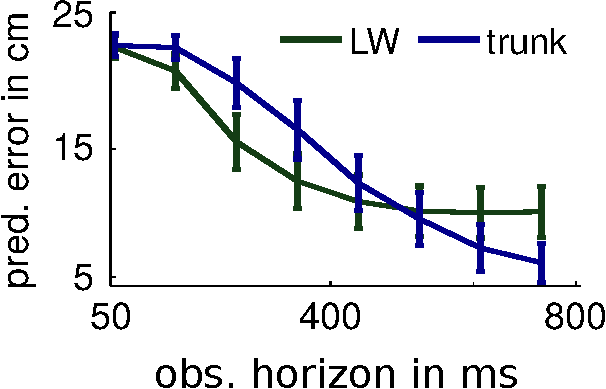
\includegraphics[width=.4\textwidth]{Elmar/picsSupp/SubFigPredErrorTrunkvsLW}
%\label{fig:subfig2}
 \caption{\textbf{Supplementary figure, Trunk vs. Left Wrist prediction error:} 
 Average prediction error in cm over all subjects given the left wrist (LW) or the trunk motion as observation. 
 }
\label{fig:SubFigPredErrorTrunkvsLW}
\end{figure}



\begin{figure}
\centering
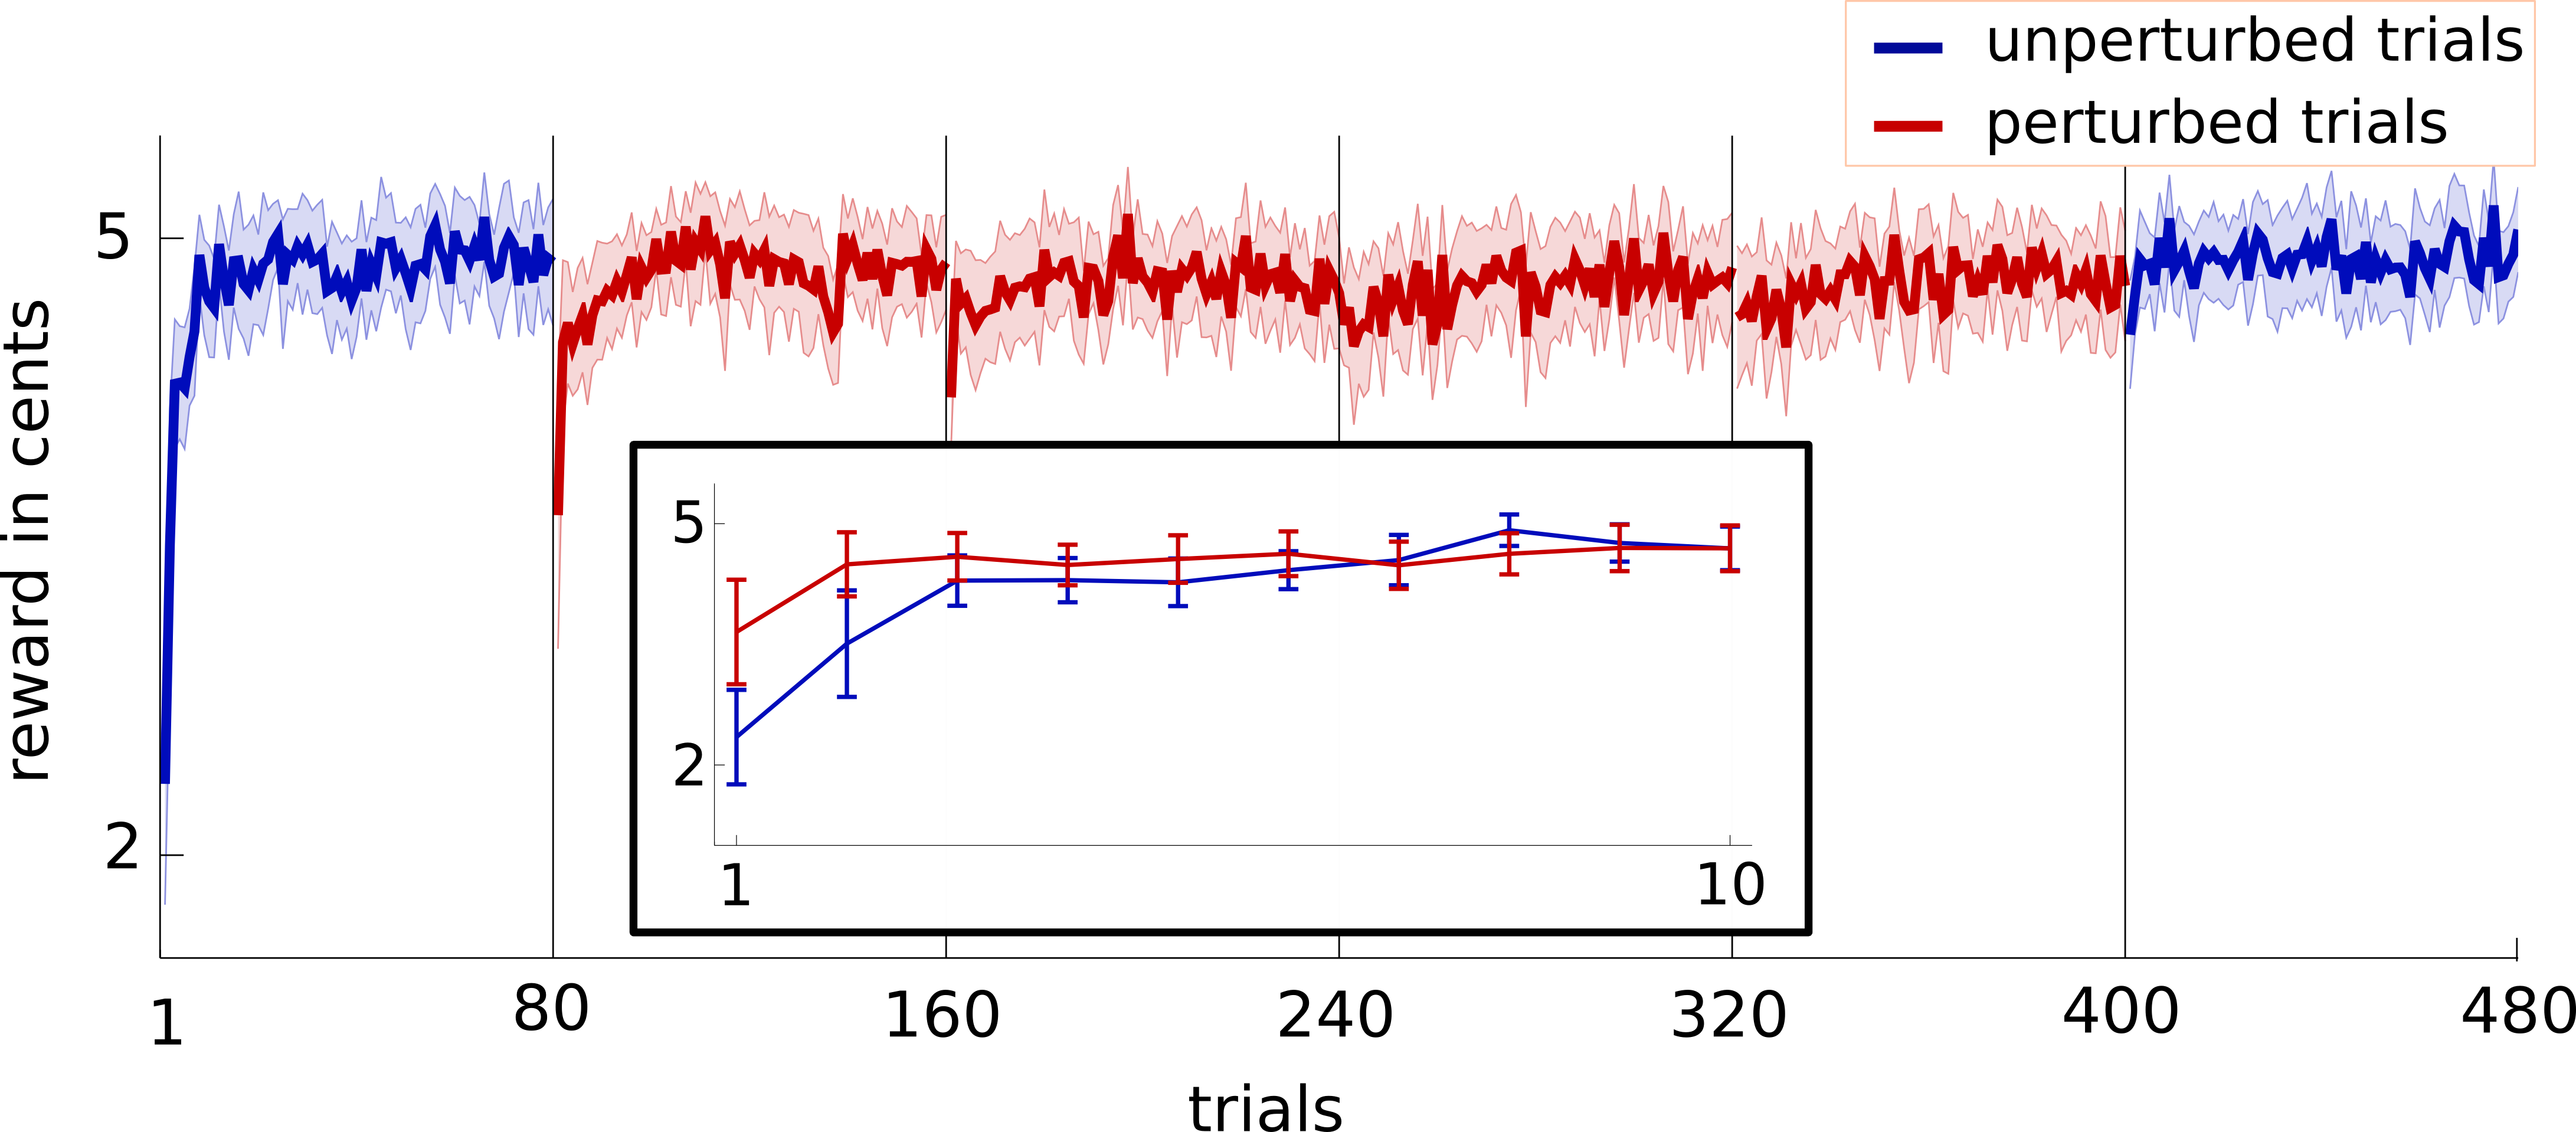
\includegraphics[width=\textwidth]{Elmar/picsSupp/FigRewards}
%\label{fig:subfig2}
 \caption{\textbf{Supplementary figure, Monetary rewards received: } 
 Illustration of the received rewards averaged over all $20$ subjects. The shaded region denotes the confidence bound. 
 }
\label{fig:SubFigRewards}
\end{figure}
